\documentclass[aspectratio=169,11pt]{beamer}

\usepackage[utf8]{inputenc}
\usepackage[T1]{fontenc}
\usepackage[spanish,es-tabla,es-nodecimaldot]{babel}
\usepackage{lmodern}
\usepackage{booktabs}
\usepackage{graphicx}
\usepackage{xcolor}

% Figuras: busca en figures/ y, si compilas desde latex/, también en ../resultados_modelo/
% y ../notebooks/resultados_modelo/ (ahí quedan protocolo_A.png y protocolo_B.png).
\graphicspath{{figures/}{./}{../figures/}{../latex/figures/}{../resultados_modelo/}{../notebooks/resultados_modelo/}}

% ---------- Resultados del protocolo B (de resumen_metricas.csv) ----------
\newcommand{\accB}{60.4}   % accuracy de prueba (%)
\newcommand{\ftB}{0.599}   % F1 macro de prueba
\newcommand{\epB}{21}      % épocas que entrenó

% ---------- Estilo (igual que la presentación del EDA) ----------
\usetheme{default}
\definecolor{acento}{HTML}{1C5CAB}
\definecolor{tinta}{HTML}{0B0B0B}
\definecolor{tinta2}{HTML}{52514E}
\definecolor{fondo2}{HTML}{F0EFEC}
\setbeamercolor{frametitle}{fg=acento}
\setbeamercolor{title}{fg=acento}
\setbeamercolor{structure}{fg=acento}
\setbeamercolor{normal text}{fg=tinta}
\setbeamercolor{block title}{bg=acento,fg=white}
\setbeamercolor{block body}{bg=fondo2}
\setbeamerfont{frametitle}{series=\bfseries,size=\Large}
\setbeamerfont{title}{series=\bfseries,size=\LARGE}
\setbeamertemplate{navigation symbols}{}
\setbeamertemplate{itemize items}[circle]
\setbeamertemplate{enumerate items}[default]
\setbeamertemplate{footline}{%
  \hspace{1em}{\color{tinta2}\tiny RAVDESS · Modelo de clasificación}\hfill
  {\color{tinta2}\tiny\insertframenumber/\inserttotalframenumber}\hspace{1em}\vspace{0.6em}}
\newcommand{\nota}[1]{{\small\color{tinta2}#1}}

\title{Reconocimiento de emociones en la voz}
\subtitle{Modelo de clasificación sobre el corpus RAVDESS (habla)}
\author{Saúl Rojas \and Karol Cisneros \and Mónica Gonzalez}
\date{\today}

\begin{document}

\begin{frame}[plain]
  \titlepage
\end{frame}

% ===================== PROBLEMA =====================
\section{Problema}
\begin{frame}{Problema}
  \begin{block}{Objetivo general}
    Clasificar la emoción expresada en un audio de voz (8 clases) con una red neuronal convolucional.
  \end{block}
  \vspace{0.6em}
  \textbf{Es un problema de clasificación multiclase}, no de regresión.
  \begin{itemize}
    \item \textbf{Entrada:} un clip de voz de $\approx$ 4 s.
    \item \textbf{Salida:} una de 8 emociones: neutral, calma, alegría, tristeza, enojo, miedo, asco, sorpresa.
    \item \textbf{Azar:} $1/8 = 12.5\,\%$ de accuracy.
  \end{itemize}
  \textbf{Objetivos específicos}
  \begin{enumerate}
    \item Construir un modelo basado en la referencia \emph{Speech Emotion Recognition 90\,\%}.
    \item Evitar la fuga de datos de la referencia (aumentar \emph{después} de dividir).
    \item Medir si el modelo generaliza a hablantes que nunca vio.
  \end{enumerate}
\end{frame}

% ===================== DATOS =====================
\section{Datos}
\begin{frame}{Datos: RAVDESS (recordatorio del EDA)}
  \small
  \begin{columns}[T]
    \begin{column}{0.5\textwidth}
      \begin{itemize}
        \item \textbf{Origen:} Livingstone y Russo (2018), CC BY-NC-SA 4.0
        \item \textbf{Tamaño:} 1440 WAV, 24 actores (12 H / 12 M), 60 clips por actor
        \item \textbf{Formato:} habla, 48 kHz, 2 frases en inglés
      \end{itemize}
    \end{column}
    \begin{column}{0.5\textwidth}
      \begin{itemize}
        \item \textbf{Etiquetas:} salen del nombre del archivo
        \item \textbf{Calidad:} sin nulos ni duplicados; 5 clips estéreo $\to$ mono
        \item \textbf{Balance:} 192 clips por emoción, salvo neutral (96)
      \end{itemize}
    \end{column}
  \end{columns}
  \vspace{0.3em}
  \centering
  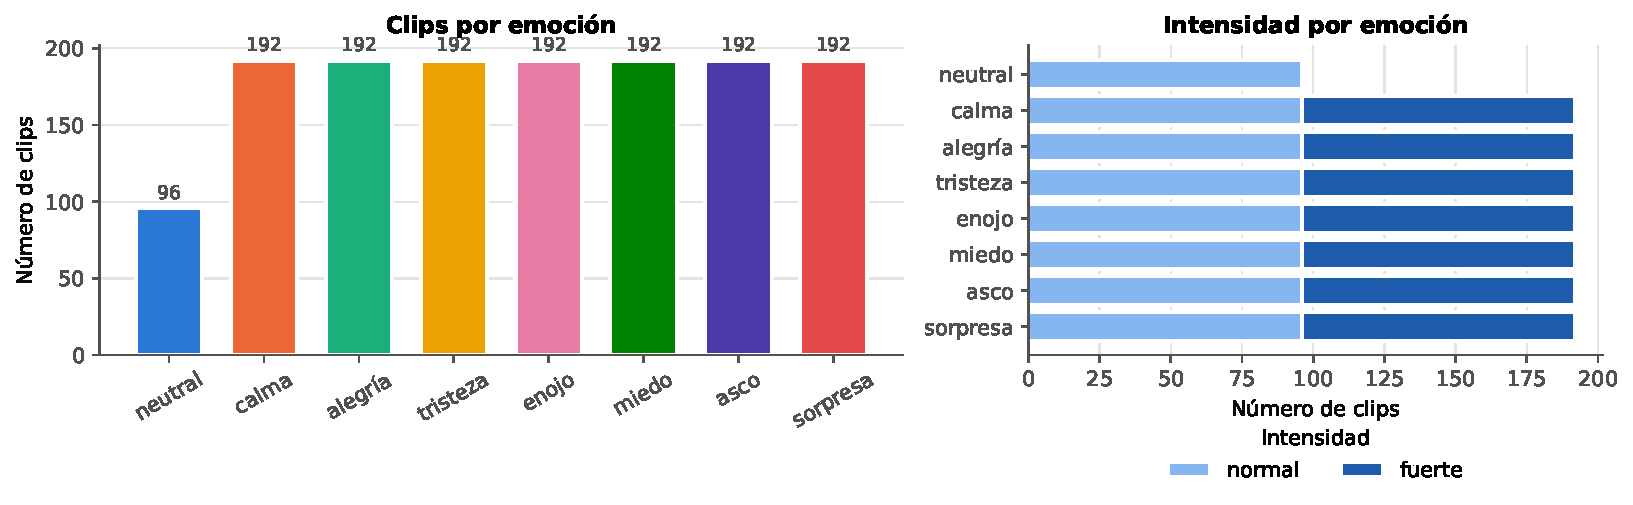
\includegraphics[width=0.92\linewidth]{distribucion_emociones}
\end{frame}

\begin{frame}{Hallazgos del EDA que condicionan el modelo}
  \begin{columns}[T]
    \begin{column}{0.5\textwidth}
      \begin{itemize}
        \item \textbf{49.8 \%} de cada clip es silencio $\Rightarrow$ solo se usan 2.5 s.
        \item Energía, F0, duración y centroide difieren por emoción (Kruskal--Wallis, $p<10^{-10}$), pero \textbf{ninguno separa las 8 clases solo}.
        \item Los atípicos de energía son señal ($\approx$ 10 \%) $\Rightarrow$ se conservan.
        \item \textbf{El hablante domina sobre la emoción:} $\Rightarrow$ hay que evaluar con actores no vistos.
      \end{itemize}
    \end{column}
    \begin{column}{0.5\textwidth}
      \centering
      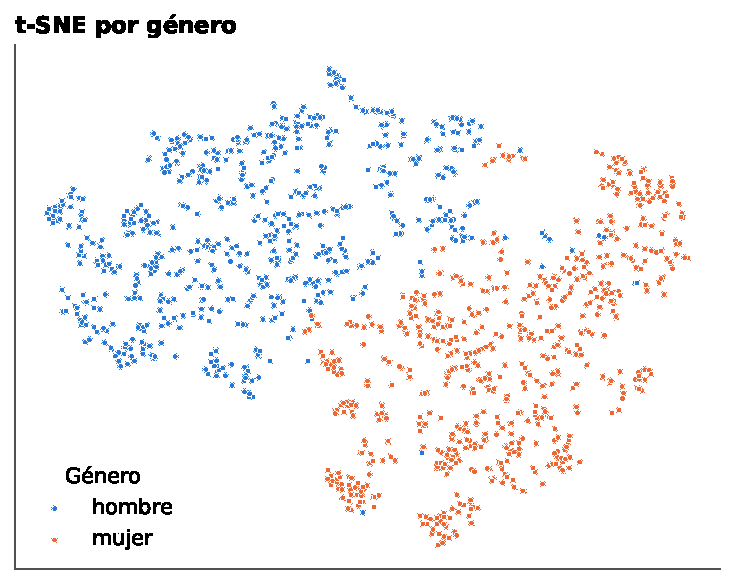
\includegraphics[width=0.9\linewidth]{tsne_genero}\\[0.3em]
      \nota{t-SNE: el género forma dos regiones casi disjuntas.}
    \end{column}
  \end{columns}
\end{frame}

% ===================== MODELO =====================
\section{Modelo}
\begin{frame}{Modelo: tratamiento de los datos}
  \begin{enumerate}
    \item \textbf{Recorte:} 2.5 s desde el segundo 0.6, a 22 050 Hz, mono.
    \item \textbf{Descriptores cuadro a cuadro} (frame 2048, hop 512 $\to$ 108 cuadros): ZCR, RMS y 20 MFCC.
    \item \textbf{Vector por clip:} $108 \times (1+1+20) = $ \textbf{2376 valores}.
    \item \textbf{Aumentación $\times 3$} (solo entrenamiento): original, + ruido, + cambio de tono (0.7 semitonos) con ruido.
    \item \textbf{Normalización:} \texttt{StandardScaler} ajustado solo con entrenamiento.
  \end{enumerate}
  \vspace{0.5em}
  \begin{block}{Diferencia clave con la referencia}
    La referencia aumenta antes de dividir: copias ruidosas de un mismo clip caen en entrenamiento y prueba
    (fuga de datos). Aquí se divide primero.
  \end{block}
\end{frame}

\begin{frame}{Modelo: arquitectura (red Conv1D)}
  \begin{columns}[T]
    \begin{column}{0.58\textwidth}
      \centering
      \begin{tabular}{lrrrr}
        \toprule
        Bloque & Filtros & Kernel & Pool & Dropout \\
        \midrule
        1 & 128 & 5 & 5 & --- \\
        2 & 128 & 5 & 5 & 0.2 \\
        3 & 64 & 5 & 5 & --- \\
        4 & 64 & 3 & 5 & 0.2 \\
        5 & 32 & 3 & 3 & 0.2 \\
        \bottomrule
      \end{tabular}\\[0.5em]
      \nota{Cada bloque: Conv1D $\to$ ReLU $\to$ BatchNorm $\to$ MaxPool.}
    \end{column}
    \begin{column}{0.42\textwidth}
      \begin{itemize}
        \item Entrada: vector de 2376 valores
        \item 5 bloques convolucionales
        \item Capa densa de \textbf{512} + BatchNorm
        \item Salida: \textbf{8} neuronas (softmax)
      \end{itemize}
      \nota{Anchos reducidos a $1/4$ por entrenar en CPU; con GPU: 512-512-256-256-128.}
    \end{column}
  \end{columns}
\end{frame}

\begin{frame}{Modelo: aprendizaje e hiperparámetros}
  \begin{columns}[T]
    \begin{column}{0.52\textwidth}
      \centering
      \begin{tabular}{ll}
        \toprule
        Parámetro & Valor \\
        \midrule
        Optimizador & Adam, $\text{lr}=10^{-3}$ \\
        Pérdida & Entropía cruzada \\
        Tamaño de lote & 64 \\
        Épocas & máx. 50 \\
        \emph{Early stopping} & paciencia 8 \\
        Reducción de lr & $\times 0.5$, paciencia 3 \\
        lr mínimo & $10^{-5}$ \\
        Semilla & 42 \\
        \bottomrule
      \end{tabular}
    \end{column}
    \begin{column}{0.48\textwidth}
      \begin{itemize}
        \item Se monitorea la \textbf{accuracy de validación}.
        \item Al final se recuperan los pesos de la \textbf{mejor época}, no los de la última.
        \item Métricas: accuracy y \textbf{F1 macro} (neutral tiene la mitad de clips).
      \end{itemize}
    \end{column}
  \end{columns}
\end{frame}

\begin{frame}{Dos protocolos de evaluación}
  \centering
  \begin{tabular}{lcc}
    \toprule
     & \textbf{A: por actor} & \textbf{B: al azar por clip} \\
    \midrule
    Entrenamiento & actores 1--18 & 80\,\% (estratificado) \\
    Validación & actores 19--20 & 10\,\% \\
    Prueba & actores 21--24 & 10\,\% \\
    Clips (entr. / val. / prueba) & 1080 / 120 / 240 & 1152 / 144 / 144 \\
    Con aumentación $\times 3$ & 3240 & 3456 \\
    \bottomrule
  \end{tabular}\\[1em]
  \begin{columns}[T]
    \begin{column}{0.48\textwidth}
      \begin{block}{A: hablantes no vistos}
        ¿Reconoce la emoción en personas nuevas? Es la medida más honesta de generalización.
      \end{block}
    \end{column}
    \begin{column}{0.48\textwidth}
      \begin{block}{B: mismos hablantes}
        ¿Reconoce la emoción en voces que ya conoce? Es comparable con la referencia, pero sin fuga.
      \end{block}
    \end{column}
  \end{columns}
\end{frame}

% ===================== RESULTADOS =====================
\section{Resultados}
\begin{frame}{Resultados: protocolo A (actores no vistos)}
  \centering
  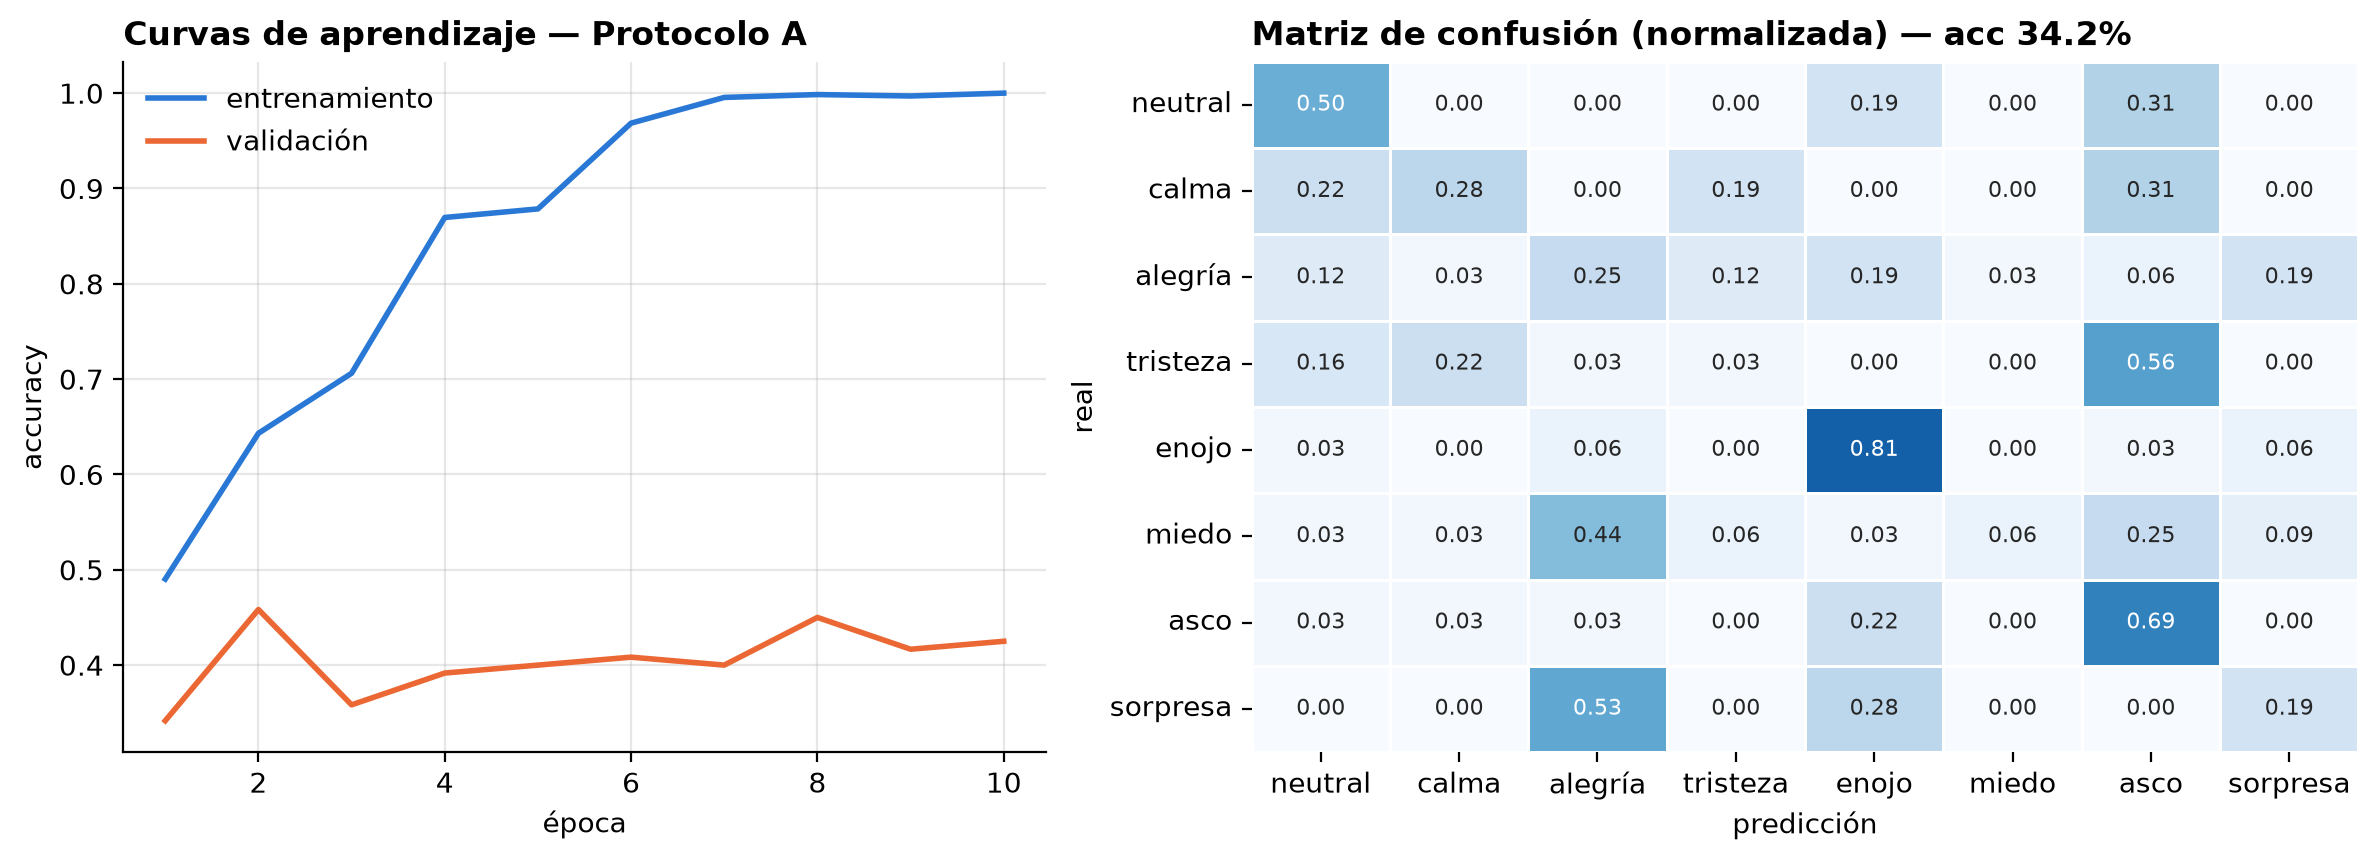
\includegraphics[width=0.93\linewidth]{protocolo_A}\\[0.3em]
  \textbf{Accuracy 43.3\,\%} y \textbf{F1 macro 0.416} sobre 240 clips (azar: 12.5\,\%).\\
  \nota{Calma se reconoce mejor (78\,\%); tristeza y miedo casi no (12\,\% cada una).}
\end{frame}

\begin{frame}{Resultados: protocolo B (división al azar)}
  \centering
  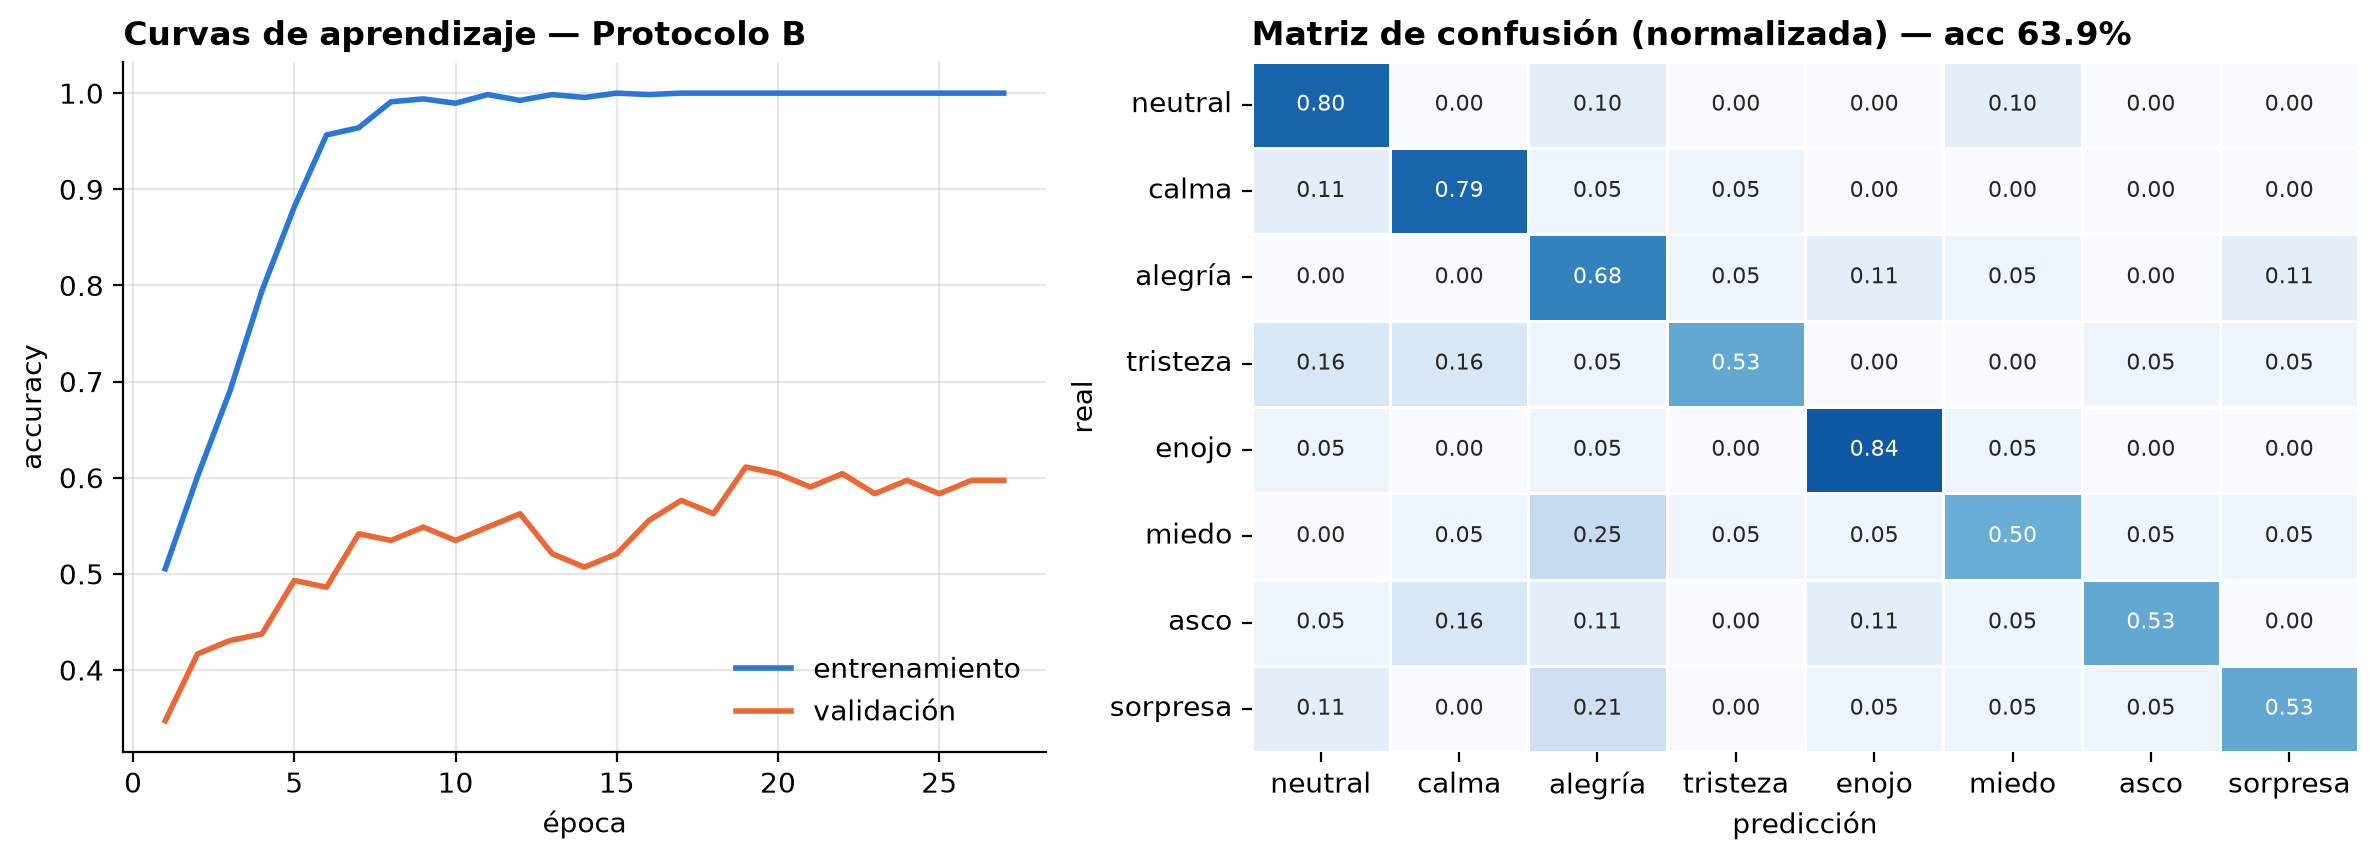
\includegraphics[width=0.93\linewidth]{protocolo_B}\\[0.3em]
  \textbf{Accuracy \accB\,\%} y \textbf{F1 macro \ftB} sobre 144 clips ($\epB$ épocas).\\
  \nota{Mejor que A porque los mismos actores aparecen en entrenamiento y prueba.}
\end{frame}

\begin{frame}{Resumen de resultados}
  \centering
  \begin{tabular}{lccc}
    \toprule
    Protocolo & Accuracy & F1 macro & Clips de prueba \\
    \midrule
    A: actores no vistos & 43.3\,\% & 0.416 & 240 \\
    B: división al azar & \accB\,\% & \ftB & 144 \\
    Azar (8 clases) & 12.5\,\% & --- & --- \\
    \bottomrule
  \end{tabular}\\[1em]
  \begin{itemize}
    \item En ambos casos el modelo \textbf{supera claramente al azar}.
    \item La brecha A--B cuantifica cuánto se apoya el modelo en \textbf{conocer al hablante}.
  \end{itemize}
\end{frame}

% ===================== DISCUSIÓN =====================
\section{Discusión}
\begin{frame}{Discusión: decisiones, éxito y limitaciones}
  \begin{columns}[T]
    \begin{column}{0.5\textwidth}
      \textbf{¿Por qué estas decisiones?}
      \begin{itemize}
        \item Recorte de 2.5 s: la mitad del clip es silencio.
        \item MFCC, ZCR y RMS: el EDA mostró que describen la activación.
        \item Dividir antes de aumentar: evita la fuga de la referencia.
        \item Protocolo A: el hablante domina sobre la emoción.
      \end{itemize}
    \end{column}
    \begin{column}{0.5\textwidth}
      \textbf{¿A qué se debe el resultado?}
      \begin{itemize}
        \item \textbf{Éxito:} 43\,\% en voces nuevas vs. 12.5\,\% del azar.
        \item \textbf{Sobreajuste:} entrenamiento llega a 1.0 y validación se queda en $\approx$ 0.4--0.5.
        \item Solo 24 actores: el modelo memoriza voces.
        \item \textbf{Confusiones:} tristeza $\to$ calma, miedo y sorpresa $\to$ alegría.
        \item En B, las 2 repeticiones de una misma actuación pueden caer en lados distintos.
      \end{itemize}
    \end{column}
  \end{columns}
\end{frame}

\begin{frame}{Conclusiones y sugerencias de mejora}
  \textbf{Conclusiones}
  \begin{enumerate}
    \item Sí hay señal emocional aprendible, pero \textbf{no generaliza bien} a hablantes nuevos con 24 actores.
    \item La cifra de la referencia ($\approx$ 90\,\%) está inflada por mezclar 4 corpus y aumentar antes de dividir.
    \item Reportar A y B juntos da una imagen honesta del desempeño.
  \end{enumerate}
  \vspace{0.4em}
  \textbf{Sugerencias}
  \begin{itemize}
    \item Más corpus y más actores (CREMA-D, TESS, SAVEE).
    \item Normalización por hablante y validación cruzada por actor.
    \item Entrenar con GPU y la red de ancho completo; probar espectrogramas o modelos preentrenados.
    \item Guardar también el \texttt{StandardScaler} para poder predecir audios nuevos.
  \end{itemize}
\end{frame}

% ===================== REFERENCIAS =====================
\begin{frame}{Referencias}
  \begin{itemize}
    \item S. R. Livingstone y F. A. Russo (2018). The Ryerson Audio-Visual Database of Emotional Speech and
      Song (RAVDESS). \emph{PLoS ONE} 13(5): e0196391. Licencia CC BY-NC-SA 4.0.
    \item B. McFee et al. (2015). librosa: Audio and music signal analysis in Python. \emph{Proc. SciPy}.
    \item gemmin. \emph{Speech Emotion Recognition 90\,\%}. Kaggle Notebook.
  \end{itemize}
\end{frame}

\end{document}
